	\documentclass[10pt,oneside]{CBFT_book}
	% Algunos paquetes
	\usepackage{amssymb}
	\usepackage{amsmath}
	\usepackage{graphicx}
	\usepackage{libertine}
	\usepackage[bold-style=TeX]{unicode-math}
	\usepackage{lipsum}

	\usepackage{natbib}
	\setcitestyle{square}

	\usepackage{polyglossia}
	\setdefaultlanguage{spanish}


	\usepackage{CBFT.estilo} % Cargo la hoja de estilo

	% Tipografías
	% \setromanfont[Mapping=tex-text]{Linux Libertine O}
	% \setsansfont[Mapping=tex-text]{DejaVu Sans}
	% \setmonofont[Mapping=tex-text]{DejaVu Sans Mono}

	%===================================================================
	%	DOCUMENTO PROPIAMENTE DICHO
	%===================================================================

\begin{document}

% =================================================================================================
\chapter{Ondas planas}
% =================================================================================================

Lejos de las fuentes de campo las ecuaciones de Maxwell son
\begin{align*}
	\divem{E} = 0 \qquad \qquad &\rotorm{E} = -\frac{1}{c}\dpar{\vb{B}}{t} \\
	\divem{B} = 0 \qquad \qquad &\rotorm{B} = \frac{1}{c}\dpar{\vb{E}}{t}
\end{align*}

Podemos derivar con respecto al tiempo en cada ecuación de rotor y reemplazar con la otra
de manera que
\[
	\rotorm{(\rotorm{B})} = \frac{1}{c}\dpar{}{t}\left(-\frac{1}{c}\dpar{\vb{B}}{t} \right)
	= \Nabla(\divem{B}) - \nabla^2 \vb{B}
\]
\[
	\rotorm{(\rotorm{E})} = -\frac{1}{c}\dpar{}{t}\left(\frac{1}{c}\dpar{\vb{E}}{t} \right)
	= \Nabla(\divem{E}) - \nabla^2 \vb{E}
\]
y esto nos lleva a 
\[
	\nabla^2 \vb{B} - \frac{1}{c^2}\dpar[2]{\vb{B}}{t} = 0 \qquad 
	\nabla^2 \vb{E} - \frac{1}{c^2}\dpar[2]{\vb{E}}{t} = 0
\]
dos sendas ecuaciones de onda para \vb{E} y \vb{B}. Pero es sabido que la solución de
\[
	\nabla^2 \psi - \frac{1}{c^2} \dpar[2]{\psi}{t} = 0
\]
es
\[
	\psi = A\euler^{i(\pe{k}{x}-\omega t)} + B\euler^{i(\pe{k}{x}-\omega t)}
\]
de modo que podemos postular como soluciones para nuestras ecuaciones de onda a
\[
	\vb{E} = \vec{\mathbb{E}}_0 \euler^{i(\pe{k}{x}-\omega t)} \qquad 
	\vb{B} = \vec{\mathbb{B}}_0 \euler^{i(\pe{k}{x}-\omega t)}
\]

Se tiene además que $\vb{k} = k \hat{n}$ da a través de $\hat{n}$ la dirección de
propagación de la onda. El número de onda $k$ podrá ser complejo lo cual refleja
atenuación. Las características del medio entran a través de
\[
	k = \sqrt{\mu\epsilon} \frac{\omega}{c}
\]
\notamargen{Acá hay que hacer las cuentas para demostrar todo esto que acá se
dice sin más.}
Por su parte $\vec{\mathbb{E}}_0$ y $\vec{\mathbb{B}}_0$ son complejos uniformes y
podrán dar desfasajes.

Al utilizar las ecuaciones de divergencia sobre las soluciones se obtiene que 
\[
	\hat{n}\cdot \vec{\mathbb{E}}_0 = 0 \qquad \hat{n}\cdot \vec{\mathbb{B}}_0 = 0
\]
de manera que las ondas se propagan perpendicularmente a los campos, por ello las
ondas electromagnéticas son transversales.

Utilizando las ecuaciones de rotor se llega a la importante relación 
\[
	\vec{\mathbb{B}}_0 = \sqrt{\mu\epsilon} \hat{n} \times \vec{\mathbb{E}}_0
\]
de modo que los vectores $\vec{\mathbb{E}}_0$ y $\vec{\mathbb{B}}_0$ también son perpendiculares.
Si el vector $\vb{k} \in \mathbb{R}$ entonces $\vec{\mathbb{E}}_0$ y $\vec{\mathbb{B}}_0$
tienen la misma fase.

En el vacío o en un medio LIH los campos \vb{E} y \vb{B} estarán en fase.
Asimismo
\[
	\vb{S} \parallel \hat{n}
\]
pues $\vb{S} \propto \pv{E}{H} $.

En un medio anisótropo $\divem{D}=\divem{}(\epsilon \vb{E}) = 0$ siendo $\epsilon$ un tensor.
Allí $\vec{\mathbb{E}}_0 \cdot \hat{n} \neq 0$ salvo que $\epsilon$ estee diagonalizado y
$\vb{E} \parallel$ al eje principal.

Notemos que $\vb{E},\vb{B}$ y $\hat{n}$ forman una terna derecha.

\subsection{Sobre complejos}



\subsection{Poynting promedio y energías promedio}


% =================================================================================================
\section{Polarización de ondas}
% =================================================================================================

\begin{figure}[htb]
	\begin{center}
	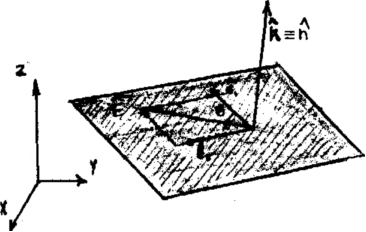
\includegraphics[width=0.4\textwidth]{images/fig_ft1_polariz.pdf}	 
	\end{center}
	\caption{}
\end{figure} 

% =================================================================================================
\section{Reflexión y refracción de ondas en medios}
% =================================================================================================

\begin{figure}[htb]
	\begin{center}
	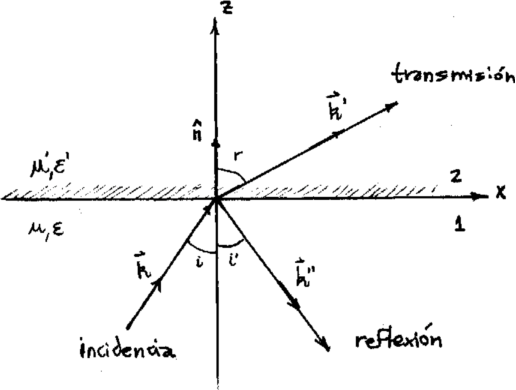
\includegraphics[width=0.4\textwidth]{images/fig_ft1_reflex1.pdf}	 
	\end{center}
	\caption{}
\end{figure} 

\begin{figure}[htb]
	\begin{center}
	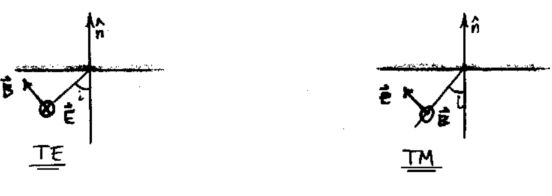
\includegraphics[width=0.4\textwidth]{images/fig_ft1_reflex2.pdf}	 
	\end{center}
	\caption{}
\end{figure} 

\begin{figure}[htb]
	\begin{center}
	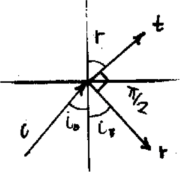
\includegraphics[width=0.4\textwidth]{images/fig_ft1_reflex3.pdf}	 
	\end{center}
	\caption{}
\end{figure} 

\begin{figure}[htb]
	\begin{center}
	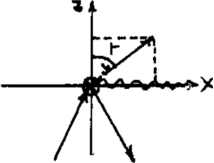
\includegraphics[width=0.4\textwidth]{images/fig_ft1_reflex4.pdf}	 
	\end{center}
	\caption{}
\end{figure} 

% =================================================================================================
\section{Campo electromagnético en un medio conductor}
% =================================================================================================

\begin{figure}[htb]
	\begin{center}
	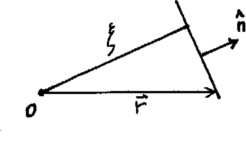
\includegraphics[width=0.4\textwidth]{images/fig_ft1_conduc1.pdf}	 
	\end{center}
	\caption{}
\end{figure} 

\begin{figure}[htb]
	\begin{center}
	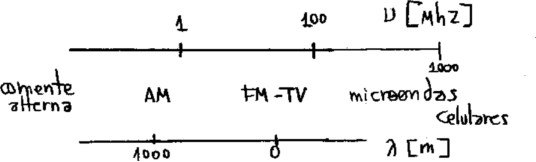
\includegraphics[width=0.4\textwidth]{images/fig_ft1_conduc2.pdf}	 
	\end{center}
	\caption{}
\end{figure} 

\begin{figure}[htb]
	\begin{center}
	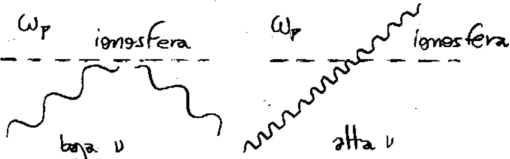
\includegraphics[width=0.4\textwidth]{images/fig_ft1_conduc3.pdf}	 
	\end{center}
	\caption{}
\end{figure} 

\begin{figure}[htb]
	\begin{center}
	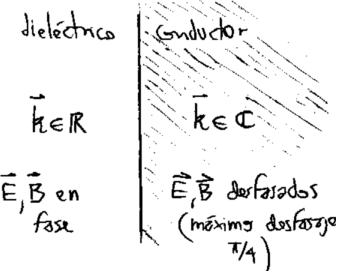
\includegraphics[width=0.4\textwidth]{images/fig_ft1_conduc4.pdf}	 
	\end{center}
	\caption{}
\end{figure} 

% =================================================================================================
\section{Transformación de vectores}
% =================================================================================================

\begin{figure}[htb]
	\begin{center}
	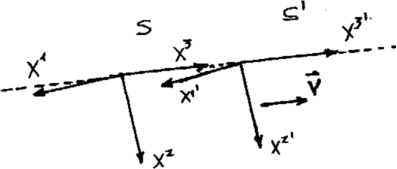
\includegraphics[width=0.4\textwidth]{images/fig_ft1_transfvec.pdf}	 
	\end{center}
	\caption{}
\end{figure} 


\subsection{Intervalos}

\begin{figure}[htb]
	\begin{center}
	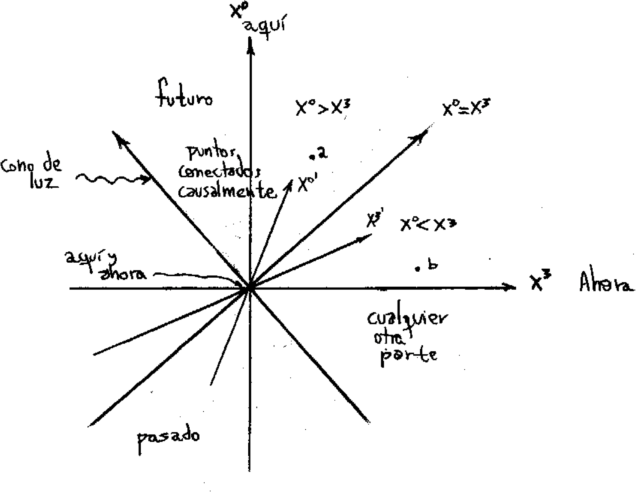
\includegraphics[width=0.4\textwidth]{images/fig_ft1_intervalos.pdf}	 
	\end{center}
	\caption{}
\end{figure} 

\subsection{Transcurso del tiempo en un sistema con V grande}

\begin{figure}[htb]
	\begin{center}
	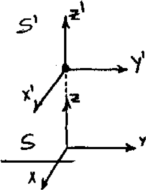
\includegraphics[width=0.4\textwidth]{images/fig_ft1_vgrande.pdf}	 
	\end{center}
	\caption{}
\end{figure} 




% \bibliographystyle{CBFT-apa-good}	% (uses file "apa-good.bst")
% \bibliography{CBFT.Referencias} % La base de datos bibliográfica

\end{document}
